\documentclass[14pt,aspectratio=1610]{beamer}
\usepackage[utf8]{inputenc}
\usepackage[ngerman]{babel}
\usetheme{simple}
%\usecolortheme{whiteonblack}
\usepackage{array}
\usepackage{tikz}
\usepackage{booktabs}
\usepackage{listings}
\usepackage{csquotes}
\usepackage{amssymb}
\newcommand{\xmark}{\ding{55}}%
\usepackage{pifont}
\newcolumntype{H}{>{\setbox0=\hbox\bgroup}c<{\egroup}@{}} % comment out columns
\author{Konrad Höffner\\Doktorand bei AKSW, BIS, Institut für Informatik \& InfAI\\Wissenschaftlicher Mitarbeiter bei IMISE (Med. Fak.)}
\title{Doktorarbeit:\\\enquote{Question Answering on RDF Data Cubes}}
%\subtitle{\small Urspünglicher Erstbetreuer: Prof. Dr. Ing. habil. Dipl.-Math. Klaus-Peter Fähnrich, Institut für Angewandte Informatik, Universität Leipzig\\~\\
%Zweitbetreuer: Prof. Dr. Jens Lehmann,\\Institut für Informatik, Universität Bonn}

\begin{document}
\begin{frame}
\titlepage
\end{frame}

%\section{PhD progress \mbox{November 2014--May 2016}}

\begin{frame}[fragile]{Domäne}
\begin{center}
\begin{tikzpicture}
  \scriptsize
  \tikzset{venn circle/.style={circle,minimum width=0.40\textwidth,fill=#1,opacity=0.4}}
  \node[venn circle = red] (SW) at (0,0) {};
  \node[venn circle = blue] (QA) at (60:0.17\textwidth) {};
  \node[venn circle = green] (QB) at (0:0.17\textwidth) {};

  \node[above,rotate=-45,yshift=-0.130\textwidth] at (barycentric cs:SW=1) {Semantic Web /  RDF};
  \node[above,yshift=0.06\textwidth] at (barycentric cs:QA=1) {Question Answering (QA)};
  \node[above,rotate=45,yshift=-0.130\textwidth] at (barycentric cs:QB=1) {Data Cube};
  \node[left,xshift=-0.050\textwidth,yshift=0.050\textwidth,align=center] at (barycentric cs:SW=1/2,QA=1/2) {SQA};
  \node[below,yshift=-0.050\textwidth,align=center] at (barycentric cs:SW=1/2,QB=1/2 ) {RDF\\Data Cube\\(RDC)};
  \node[right,yshift=0.05\textwidth] at (barycentric cs:QA=1/2,QB=1/2 ) {~};
  \node[below,yshift=0.025\textwidth] at (barycentric cs:SW=1/3,QA=1/3,QB=1/3 ){RDCQA};
\end{tikzpicture}
\end{center}
\end{frame}

\begin{frame}[fragile]{Projekte}
\centering
\begin{center}
\begin{tikzpicture}
  \scriptsize
  \tikzset{venn circle/.style={circle,minimum width=0.40\textwidth,fill=#1,opacity=0.4}}
  \node[venn circle = red] (SW) at (0,0) {};
  \node[venn circle = blue] (QA) at (60:0.17\textwidth) {};
  \node[venn circle = green] (QB) at (0:0.17\textwidth) {};

  \node[above,rotate=-45,yshift=-0.130\textwidth] at (barycentric cs:SW=1) {Semantic Web / RDF};
  \node[above,yshift=0.06\textwidth] at (barycentric cs:QA=1) {Question Answering (QA)};
  \node[above,rotate=45,yshift=-0.130\textwidth] at (barycentric cs:QB=1) {Data Cube};
  \node[left,xshift=-0.050\textwidth,yshift=0.050\textwidth,align=center] at (barycentric cs:SW=1/2,QA=1/2) {SQA\\\textbf{1. Survey}};
  \node[below,yshift=-0.050\textwidth,align=center] at (barycentric cs:SW=1/2,QB=1/2 ) {RDF\\Data Cube\\(RDC)\\\textbf{3. LinkedSpending}};
  \node[right,yshift=0.05\textwidth] at (barycentric cs:QA=1/2,QB=1/2 ) {~};
  \node[below,yshift=0.025\textwidth] at (barycentric cs:SW=1/3,QA=1/3,QB=1/3 ){RDCQA \textbf{2. CubeQA}};
\end{tikzpicture}
\end{center}
\end{frame}

\begin{frame}{Survey on Challenges of Question Answering in the Semantic Web}
\begin{itemize}
\item Systematische Untersuchung von SQA Systemen
\item SQA: Semantic Question Answering (Question Answering auf RDF Daten)
\item 1960 Kandidaten, 62 Systeme, 72 Publikationen
\item Kategorizierung nach Problemen, wie Lexical Gap, Mehrdeutigkeit, Mehrsprachigkeit
\item Sammlung von etablierten Methoden und Lösungsansätzen für die Zukunft
\end{itemize}
\end{frame}

\begin{frame}{LinkedSpending: OpenSpending becomes Linked Open Data}
\begin{itemize}
\item OpenSpending: \enquote{Mapping the money}
\item Finanztransaktionen von Regierungen weltweit in Data Cubes
\item LinkedSpending: Konvertierung der Data Cubes nach RDF Data Cubes 
\end{itemize}
\end{frame}

\begin{frame}{RDF Data Cube Vokabular}
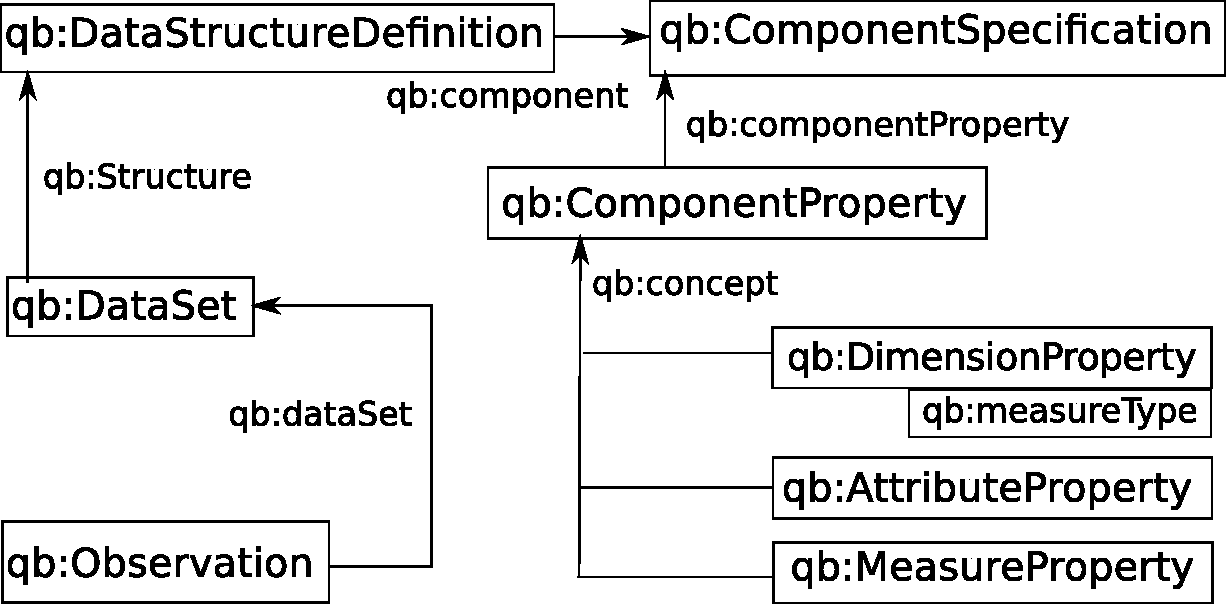
\includegraphics[width=\textwidth]{img/rdfdatacube_shrinked.pdf}
\end{frame}

\begin{frame}{Veröffentlichung}
\begin{itemize}
\item Webseite: \url{http://linkedspending.aksw.org}
\item SPARQL Endpunkt: \url{http://linkedspending.aksw.org/sparql}
\end{itemize}
\end{frame}


\begin{frame}{CubeQA:\\Question Answering on RDF Data Cubes }
\begin{itemize}
\item vereint alle Forschungsgebiete: Semantic Web, Question Answering \& Data Cubes
\item Neues Unterforschungsgebiet von Question Answering
\item Benutzer geben vollständige englische Fragen ein.
\item Frage wird in SPARQL Query auf RDF Data Cubes transformiert.
\item Operationen von Data Cubes werden unterstützt, z.B. Dice und Slice. 
\end{itemize}
\end{frame}

\begin{frame}{Beispielfrage}
\centering\large
How much did the Philippines receive in the years of 2007 to 2008?
\end{frame}

\begin{frame}{Aussschnitt aus dem Data Cube "Finland Aid"}
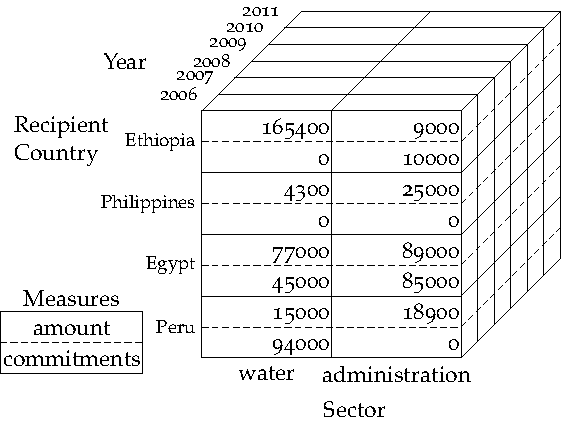
\includegraphics[width=0.85\textwidth]{img/datacube-full.pdf}
\end{frame}

\begin{frame}{Operation: Dice}
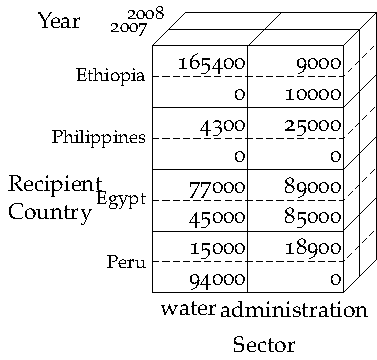
\includegraphics[width=0.65\columnwidth]{img/datacube-dice.pdf}
\end{frame}

\begin{frame}{Operation: Slice}
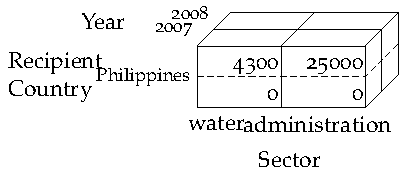
\includegraphics[width=0.65\columnwidth]{img/datacube-slice.pdf}
\end{frame}


\begin{frame}{CubeQA: Algorithmus mit einer Pipeline}
\centering
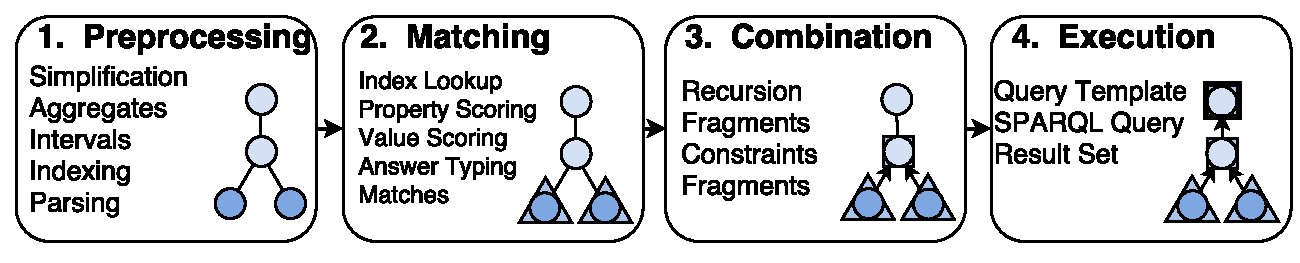
\includegraphics[width=\columnwidth]{img/cubeqapipeline-numbered.pdf}
\end{frame}

\begin{frame}[fragile]{CubeQA: SPARQL Query}
\small
\begin{lstlisting}[language=sparql]
PREFIX :<http://linkedspending.aksw.org/instance/finland-aid/>
SELECT sum(xsd:decimal(?amount))
FROM <http://linkedspending.aksw.org/finland-aid>                                                                                                                                                                  
{
 ?o a qb:Observation.
 ?o lso:finland-aid-amount ?amount.
 ?o lso:finland-aid-recipient-country
    <https://openspending.org/finland-aid/recipient-country/ph>.
 ?o lso:refYear ?y.
 filter(year(?y)=2007 OR year(?y)=2008)
}
\end{lstlisting}
Ergebnis: 1\,134\,377 (\$)
\end{frame}

\begin{frame}{Doktorarbeit}
\begin{itemize}
\item Status: Finale Korrekturen
\item 167 Seiten: 120 Hauptteil, 47 Anhang
\item Urspünglicher Erstbetreuer: Prof. Dr. Ing. habil. Dipl.-Math. Klaus-Peter Fähnrich, Institut für Angewandte Informatik, Universität Leipzig
\item Zweitbetreuer: Prof. Dr. Jens Lehmann, Institut für Informatik, Universität Bonn
\end{itemize}
\end{frame}


\begin{frame}{Kernpublikationen}
\begin{tabular}{lll}
LinkedSpending \cite{linkedspending}	&Semantic Web Journal	&2014\\
SQA Survey \cite{qasurvey}		&Semantic Web Journal	&2017\\
CubeQA Short \cite{cubeqashort}		&SEMANTiCS		&2014\\
CubeQA Long \cite{cubeqa}		&ISWC			&2016\\
\end{tabular}
\\~\\~\\14 andere Publikationen (2 davon Erstauthor).
\end{frame}

\begin{frame}[allowframebreaks]{Bibliographie Kernpublikationen}
\bibliographystyle{unsrt}
\bibliography{konrad}
\end{frame}

\end{document}
